\documentclass[]{article}
\usepackage[utf8]{inputenc}                                               %% si può scegliere anche latin1, ma lo si sconsiglia 

\usepackage{comment}
\usepackage[T1]{fontenc}
\usepackage{lmodern}
%\usepackage{mhchem}                                                       %% Per scrivere formule di chimica	  
\usepackage{amsmath}                                                      %% per la matematica estesa
\usepackage{lipsum}                                                       %% Per scrivere testo fasullo in "latinorum"
%%\usepackage{natbib}
\usepackage[output-decimal-marker={,}]{siunitx}                                                      %% Per scrivere con le unità di misura
\usepackage{booktabs}                                                                          %% del Sistema Internazionale
\usepackage{latexsym}
\usepackage{csquotes} % per fare citazioni centrate

\usepackage{graphicx}
\usepackage{epstopdf}
\usepackage{caption}
\usepackage{subfig}
\usepackage{pdfpages}
\usepackage{wrapfig}
\usepackage{subfig}
%opening
\title{Convertitore di figure da eps a pdf}
\author{Riccardo Tessarin}

\begin{document}

\maketitle

\begin{abstract}
File usato per convertire le figure caricate in eps in pdf da inserire poi nel progetto di laurea. 
\end{abstract}

\section{Stampa delle figure}

\begin{figure}
	\centering
	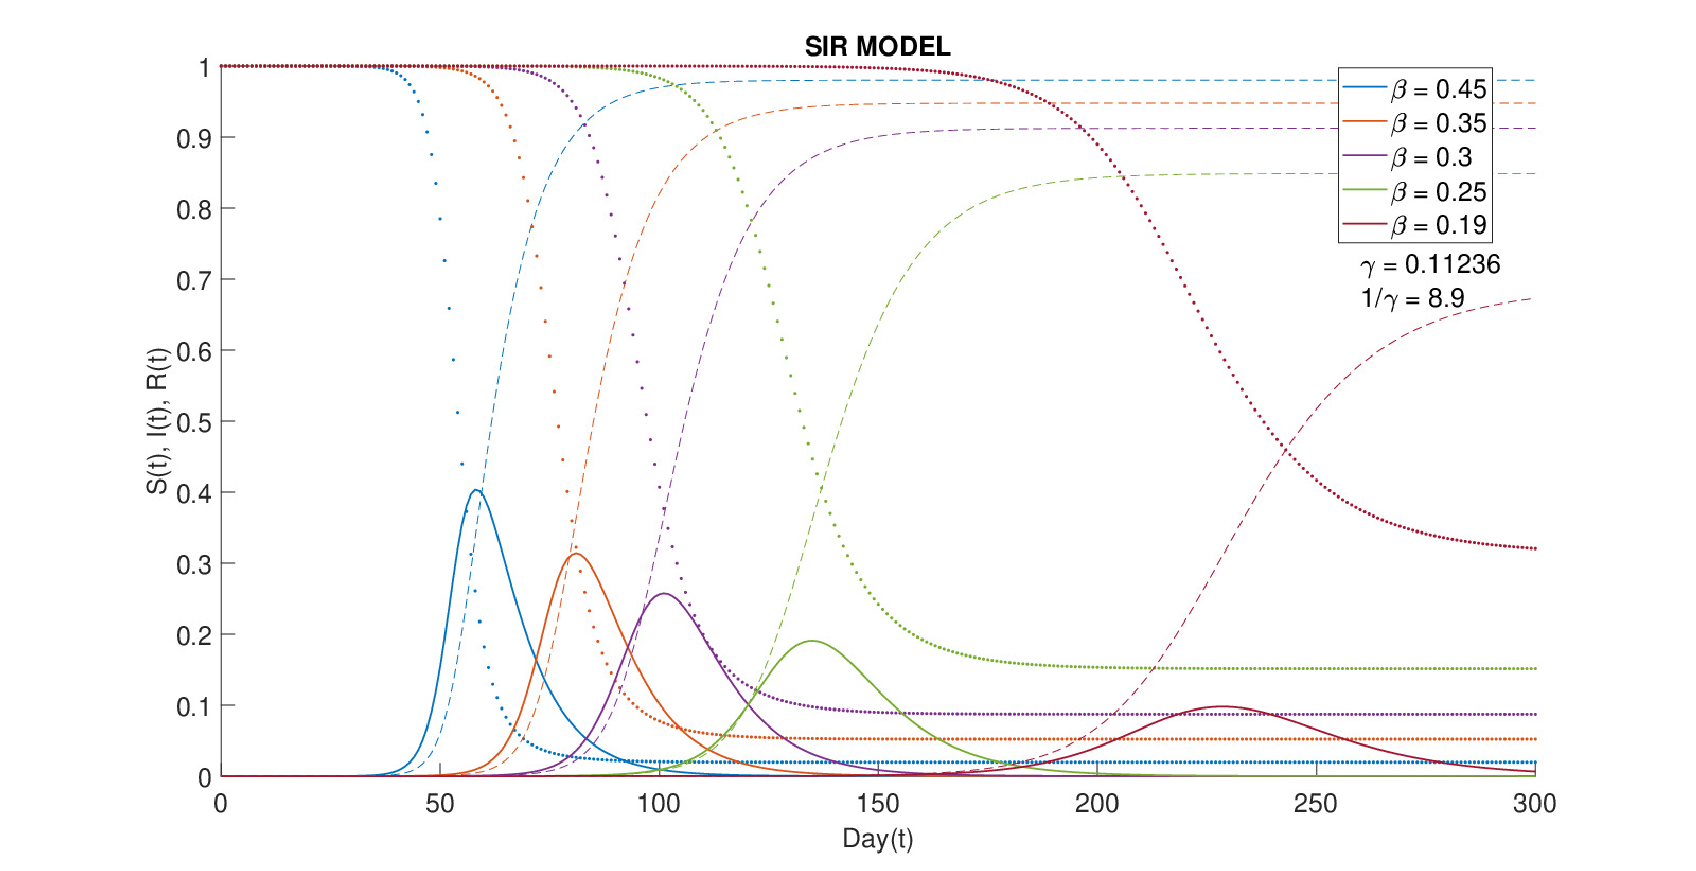
\includegraphics[width=1\linewidth]{sir_con_rt}
	\caption{}
	\label{fig:sirconrt}
\end{figure}
\begin{figure}
	\centering
	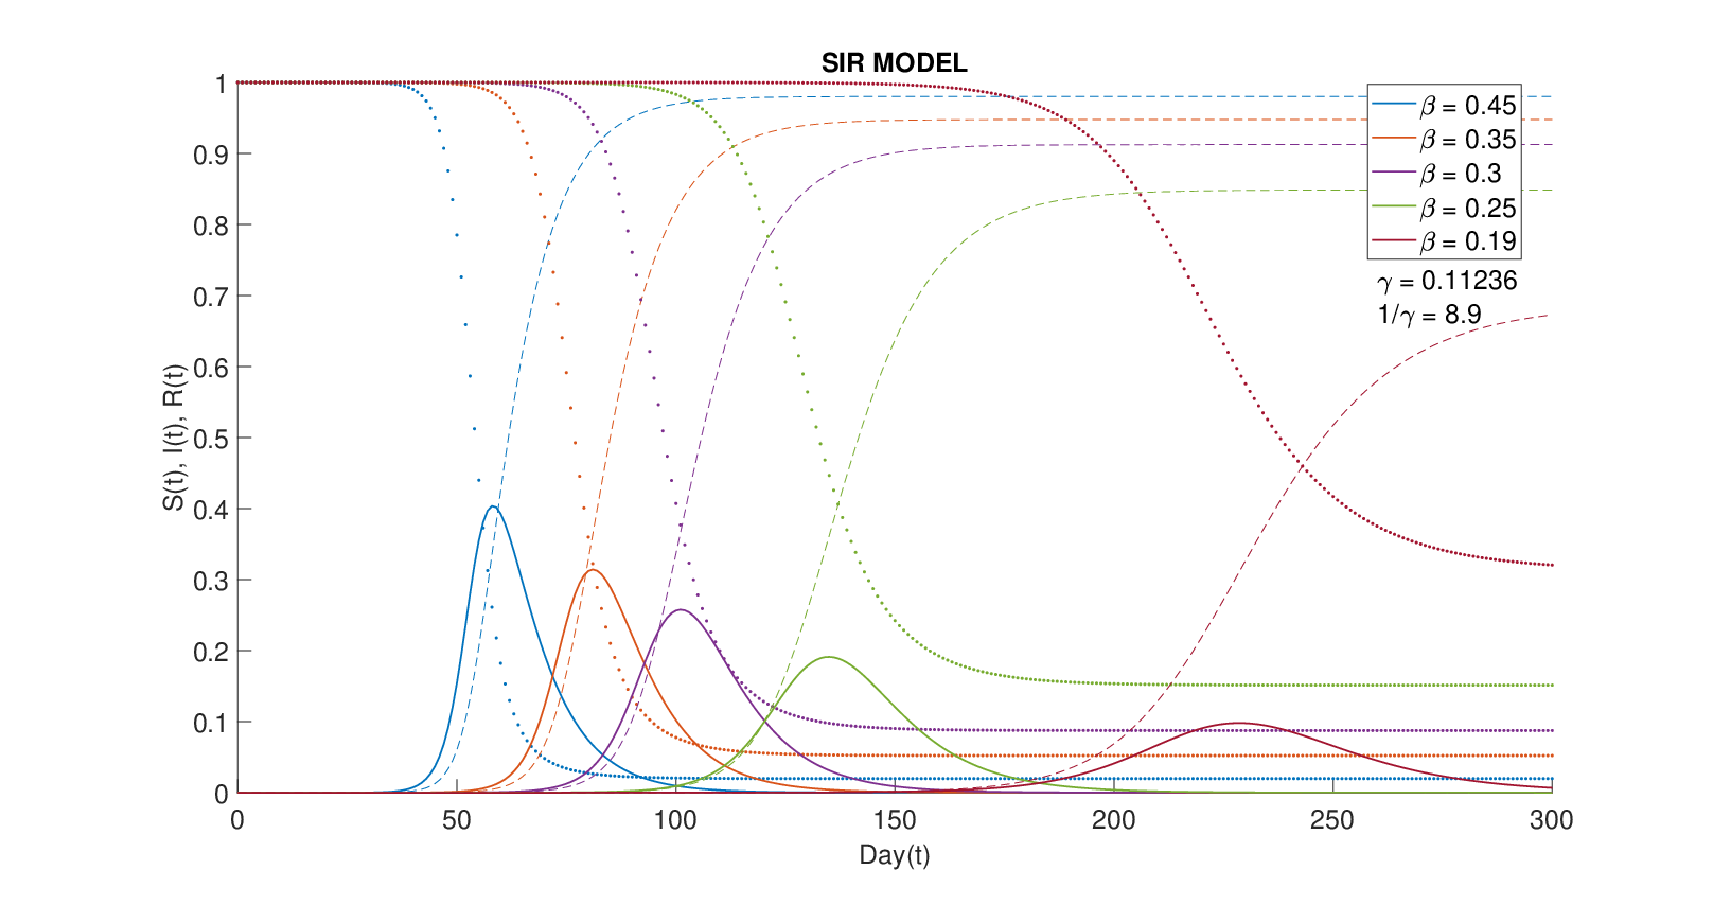
\includegraphics[width=1\linewidth]{sir_multipli_beta}
	\caption{}
	\label{fig:sirmultiplibeta}
\end{figure}



\end{document}
